\documentclass{beamer}

\usepackage{alltt}%
\usetheme{Boadilla}
\usecolortheme{seahorse}

%\usepackage{listings}
\makeatletter
\def\maxwidth{ %
  \ifdim\Gin@nat@width>\linewidth
    \linewidth
  \else
    \Gin@nat@width
  \fi
}
\makeatother

\definecolor{fgcolor}{rgb}{0.345, 0.345, 0.345}
\newcommand{\hlnum}[1]{\textcolor[rgb]{0.686,0.059,0.569}{#1}}%
\newcommand{\hlstr}[1]{\textcolor[rgb]{0.192,0.494,0.8}{#1}}%
\newcommand{\hlcom}[1]{\textcolor[rgb]{0.678,0.584,0.686}{\textit{#1}}}%
\newcommand{\hlopt}[1]{\textcolor[rgb]{0,0,0}{#1}}%
\newcommand{\hlstd}[1]{\textcolor[rgb]{0.345,0.345,0.345}{#1}}%
\newcommand{\hlkwa}[1]{\textcolor[rgb]{0.161,0.373,0.58}{\textbf{#1}}}%
\newcommand{\hlkwb}[1]{\textcolor[rgb]{0.69,0.353,0.396}{#1}}%
\newcommand{\hlkwc}[1]{\textcolor[rgb]{0.333,0.667,0.333}{#1}}%
\newcommand{\hlkwd}[1]{\textcolor[rgb]{0.737,0.353,0.396}{\textbf{#1}}}%
\let\hlipl\hlkwb

\usepackage{framed}
\makeatletter
\newenvironment{kframe}{%
 \def\at@end@of@kframe{}%
 \ifinner\ifhmode%
  \def\at@end@of@kframe{\end{minipage}}%
  \begin{minipage}{\columnwidth}%
 \fi\fi%
 \def\FrameCommand##1{\hskip\@totalleftmargin \hskip-\fboxsep
 \colorbox{shadecolor}{##1}\hskip-\fboxsep
     % There is no \\@totalrightmargin, so:
     \hskip-\linewidth \hskip-\@totalleftmargin \hskip\columnwidth}%
 \MakeFramed {\advance\hsize-\width
   \@totalleftmargin\z@ \linewidth\hsize
   \@setminipage}}%
 {\par\unskip\endMakeFramed%
 \at@end@of@kframe}
\makeatother

\definecolor{shadecolor}{rgb}{.97, .97, .97}
\definecolor{messagecolor}{rgb}{0, 0, 0}
\definecolor{warningcolor}{rgb}{1, 0, 1}
\definecolor{errorcolor}{rgb}{1, 0, 0}
\newenvironment{knitrout}{}{} % an empty environment to be redefined in TeX


\usepackage[utf8]{inputenc}
\usepackage{default}

\usepackage{xcolor}%for color mixing

\usepackage{amsmath}%
\usepackage{amsfonts}%
\usepackage{amssymb}%
\usepackage{graphicx}


\setbeamertemplate{itemize/enumerate body begin}{\small}

%%%%%%%%%%%%%%%%%%%%%%%%%%%%%%%%%%%%%%%%%%%%%%%%%%%%%%%%%%%%%%%%%%%%%%%%%%%%%%%%%%

\title{Statisitcal Thinking in Biology Research}
\author{Terry Neeman and Timothee Bonnet}
\date{\today}

\begin{document}

%\lstset{language=R}%code

\AtBeginSection[]
{
  \begin{frame}<beamer>
    \frametitle{}
    \tableofcontents[currentsection,sectionstyle=show/show,subsectionstyle=show/shaded/hide]% down vote\tableofcontents[currentsection,currentsubsection,hideothersubsections,sectionstyle=show/hide,subsectionstyle=show/shaded/hide] 
  \end{frame}
}


\begin{frame}{}
\maketitle

\end{frame}
%%%%%%%%%%%%%%%%%%%%%%%

\begin{frame}{Acknowledgemnts and warning}

\end{frame}
%%%%%%%%%%%%%%%%%%%%%%%

\begin{frame}{Key ideas for today}

\begin{itemize}[<+->]
 \item Statistics in biology is the study of biological variation
 \item Statistical ideas about biological variation inform the design of experiments
 \item Statistical ideas about biological variation inform the analysis of experiments
 \item Statistical thinking is an essential component of scientific thinking
\end{itemize}

\end{frame}
%%%%%%%%%%%%%%%%%%%%%%%

\begin{frame}{A bit of history of statistical methods}
 
 R.A. Fisher: 1890-1962
 \only<1>{\begin{center}
  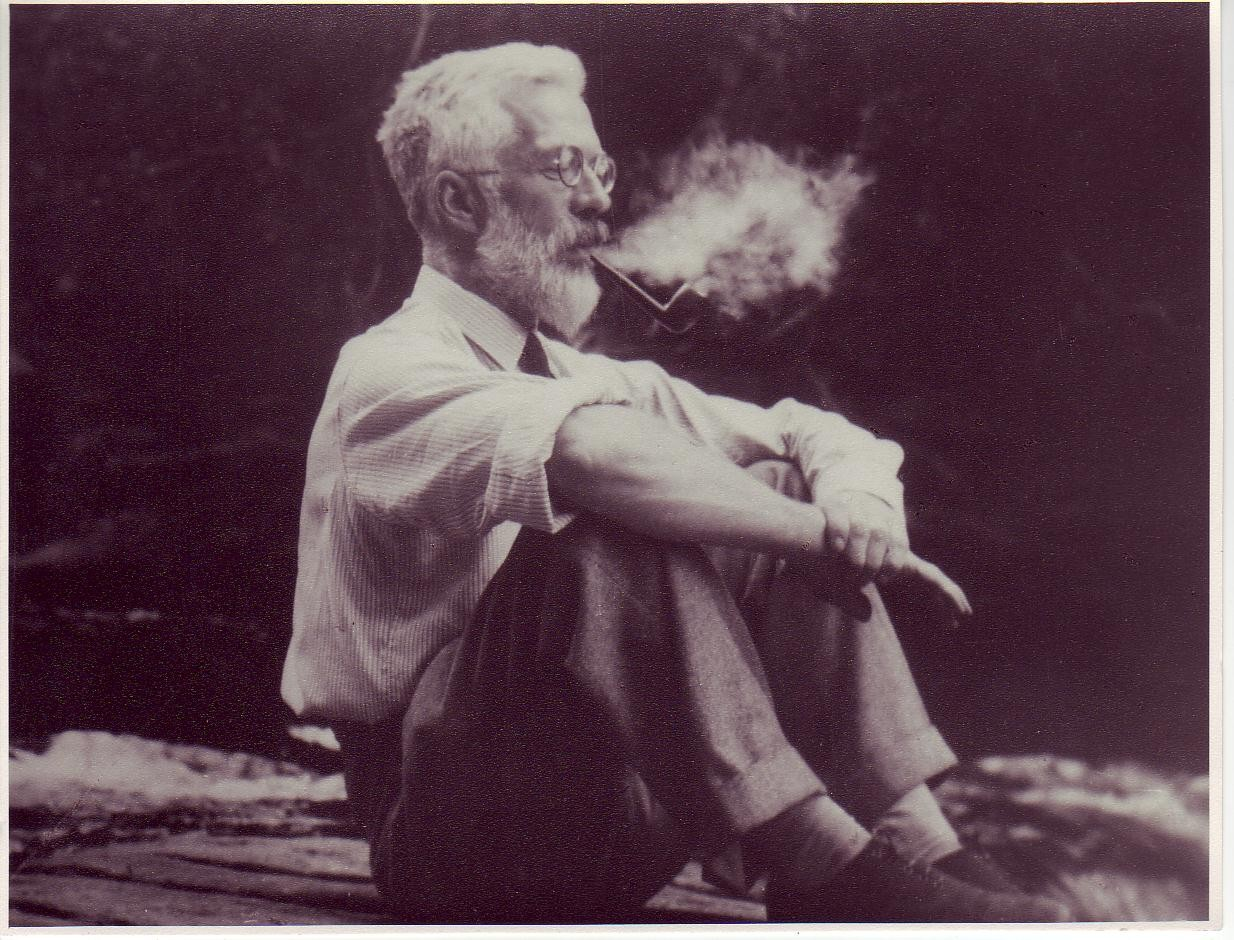
\includegraphics[width=0.5\textwidth]{Figures/fisher}
 \end{center}}
 
 \only<2>{\begin{center}
  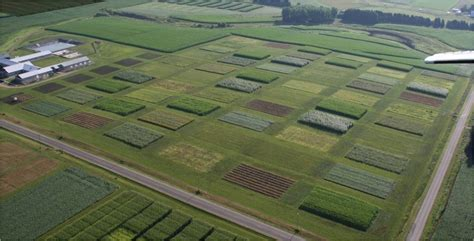
\includegraphics[width=0.9\textwidth]{Figures/fields}
 \end{center}}
 
 Statistical Principles for Research Workers (1925)

\end{frame}
%%%%%%%%%%%%%%%%%%%%%%%

%%%%%%%%%%%%%%%%%%%%%%%%%%%%%%%%%%%%%%%%%%%%%%%%%%%%%%%%%%%%%%%%%%%%%%%%%%%%%%%%%%%%%%%%%%%%%%%%%%%%%%%%%%%%%%%%%%%%
\section{Cautionary tales from the front}

%%%%%%%%%%%%%%%%%%%%%%%

\begin{frame}{Message 1: A small p-value is not always evidence of a treatment effect}

  \begin{columns}
    \begin{column}{0.5\textwidth}
	\begin{center}
	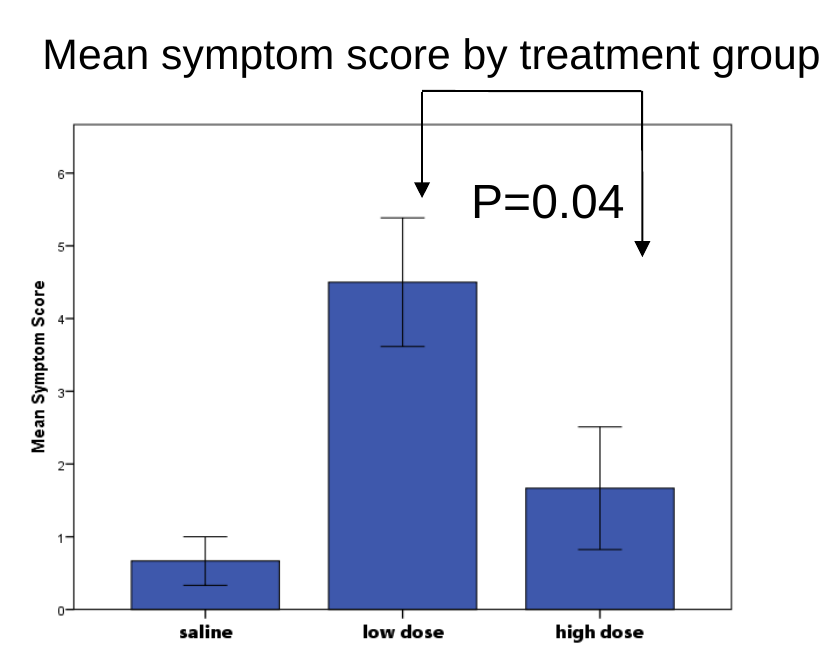
\includegraphics[width=\textwidth]{Figures/message1}
	\end{center}
    \end{column}
    
    \begin{column}{0.5\textwidth}
    \begin{block}{Vaccine challenge experiment:}
      \begin{itemize} 
       \item 6 mice/group (saline/low dose/high dose)
       \item All mice challenged with Shigella
       \item Followed for 14 days
       \item  Outcome: Symptom score average Days 2 - 8
      \end{itemize}
      \end{block}
      
      \begin{alertblock}{}
       One-way ANOVA (post-hoc Bonferroni) p=0.04
      \end{alertblock}

    \end{column}
  \end{columns}
  
  \pause \vspace{0.3cm}
  \emph{\large Do you think the vaccine works? What is strange?}
  

\end{frame}
%%%%%%%%%%%%%%%%%%%%%%%

\begin{frame}{Message 1: A small p-value is not always evidence of a treatment effect}
\pause
 \vspace{-0.2cm}
 \begin{center}
  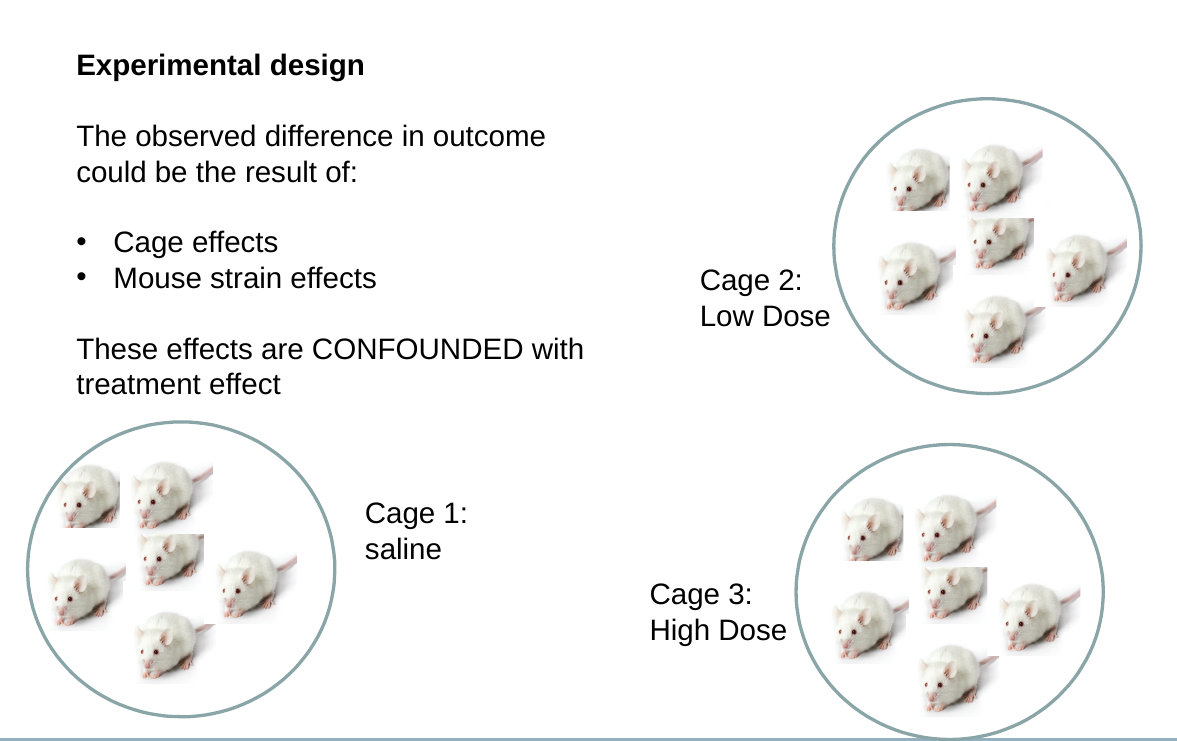
\includegraphics[width=\textwidth]{Figures/mice}
 \end{center}
 
\end{frame}
%%%%%%%%%%%

\begin{frame}{Message 2: p-values from simple comparisons cannot tell us when differences are “different”}
 \pause
  \begin{columns}
    \begin{column}{0.5\textwidth}
	\begin{center}
	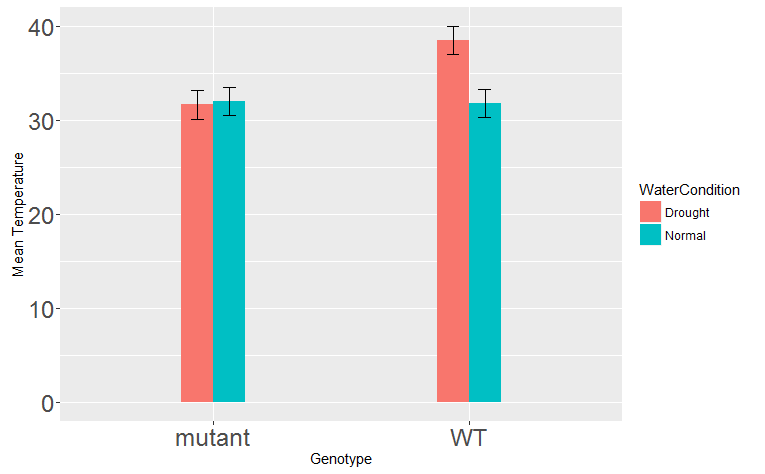
\includegraphics[width=\textwidth]{Figures/message2}
	\end{center}
    \end{column}
    
    \begin{column}{0.5\textwidth}
    \begin{block}{Are temperature mechanisms modified in a genetically modified tomato plant?}
      \begin{itemize}
	\item Genotypes: WT/mutant 
	\item Water condition: Normal/Drought
	\item Leaf temperature measured
      \end{itemize}
      \end{block}
  
    \end{column}
  \end{columns}
   
   
   \begin{alertblock}{Comparisons made using t-tests}
Evidence of difference + No evidence of difference $\neq$ Evidence that differences are different.
      \end{alertblock}
      
      
\end{frame}
%%%%%%%%%%%


\begin{frame}{Message 3: Interpreting experimental results needs more than t-tests}
 \pause
 Research question: Are mice susceptible to obesity when exposed to a high fat diet?
 
  \begin{columns}
    \begin{column}{0.5\textwidth}
	\begin{center}
	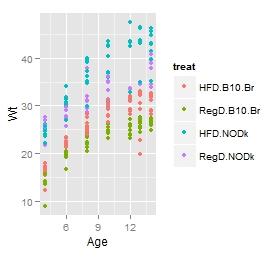
\includegraphics[width=\textwidth]{Figures/message3}
	\end{center}
    \end{column}
    
    \begin{column}{0.5\textwidth}
    \begin{block}{Experimental set-up:}
      \begin{itemize}
	\item 37 mice: 16 NODk /21 WT
	\item Randomised to either regular or high fat diet
	\item Monitored for 14 weeks
	\item Outcome measure: Body weight (g)
	\item Experimental factors: Diet (2), Strain (2), Time (8)
      \end{itemize}
      \end{block}
      \tiny Acknowledgements: Ainy Hussain, PhD student 2013
    \end{column}
  \end{columns}
   
\end{frame}
%%%%%%%%%%%

\begin{frame}{Message 4: Knowing how to combine information across subgroups  can improve inference}
 
 \pause 
 
 Comparing yield in five barley varieties (1930s) \\
 Experimental factors: 5 varieties of barley, 6 locations, 2 time points. Outcome measure: yield
  \begin{columns}
    \begin{column}{0.6\textwidth}
	\begin{center}
	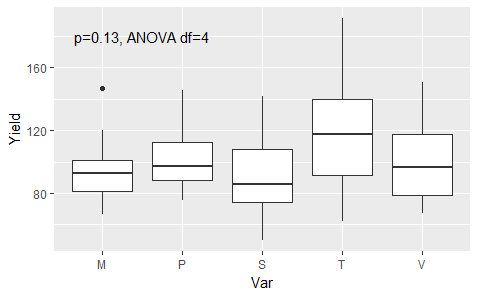
\includegraphics[width=\textwidth]{Figures/message4a}
	\end{center}
    \end{column}
    
    \begin{column}{0.4\textwidth}
  
    \end{column}
  \end{columns}
      \tiny Acknowledgements: MASS R-package
   
\end{frame}
%%%%%%%%%%%


\begin{frame}{Message 4: Knowing how to combine information across subgroups  can improve inference}
 
  
 Comparing yield in five barley varieties (1930s) \\
 Experimental factors: 5 varieties of barley, 6 locations, 2 time points. Outcome measure: yield
  \begin{columns}
    \begin{column}{0.5\textwidth}
	\begin{center}
	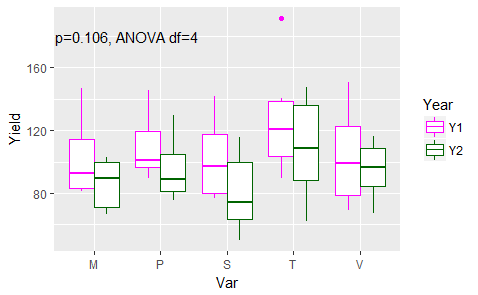
\includegraphics[width=\textwidth]{Figures/message4b}
	\end{center}
    \end{column}
    
    \begin{column}{0.5\textwidth}
    \begin{block}{Controlling for other sources of variation:}
      \begin{itemize}
	\item Controlling for year = comparing yield WITHIN years and combining these
      \end{itemize}
      \end{block}
      \tiny Acknowledgements: MASS R-package
    \end{column}
  \end{columns}
   
\end{frame}
%%%%%%%%%%%


\begin{frame}{Message 4: Knowing how to combine information across subgroups  can improve inference}
 
  
 Comparing yield in five barley varieties (1930s) \\
 Experimental factors: 5 varieties of barley, 6 locations, 2 time points. Outcome measure: yield
  \begin{columns}
    \begin{column}{0.5\textwidth}
	\begin{center}
	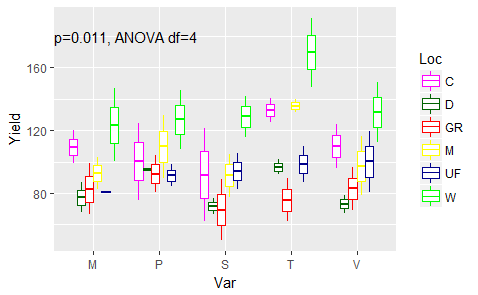
\includegraphics[width=\textwidth]{Figures/message4c}
	\end{center}
    \end{column}
    
    \begin{column}{0.5\textwidth}
    \begin{block}{Controlling for other sources of variation:}
      \begin{itemize}
	\item Control for year = compare yield WITHIN years and combine these
	\item Control for location = compare yield WITHIN locations and combine these
      \end{itemize}
      \end{block}
      \tiny Acknowledgements: MASS R-package
    \end{column}
  \end{columns}
   
\end{frame}
%%%%%%%%%%%


\begin{frame}{Message 4: Knowing how to combine information across subgroups  can improve inference}
 
  \begin{columns}
    \begin{column}{0.5\textwidth}
	\begin{center}
	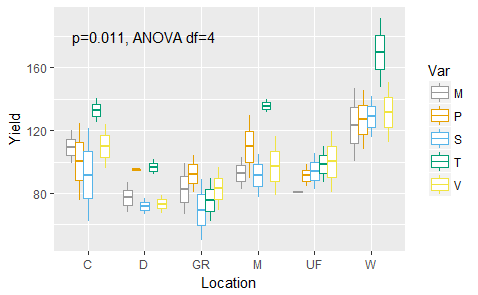
\includegraphics[width=\textwidth]{Figures/message4d}
	\end{center}
    \end{column}
    
    \begin{column}{0.5\textwidth}
    \begin{block}{Controlling for other sources of variation:}
      \begin{itemize}
	\item Control for year = compare yield WITHIN years and combine these
	\item Control for location = compare yield WITHIN locations and combine these
      \end{itemize}
      \end{block}
      \tiny Acknowledgements: MASS R-package
    \end{column}
  \end{columns}
   
\end{frame}
%%%%%%%%%%%


\begin{frame}{Message 5: Knowing what factors contribute to the variation in outcome helps design experiments and analyses}
 \pause
 Research question: 
How does cold duration impact upon germination in alpine plant A. glacialis?

  \begin{columns}
    \begin{column}{0.5\textwidth}
	\begin{center}
	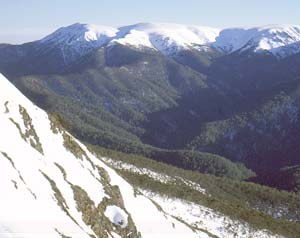
\includegraphics[width=\textwidth]{Figures/message5}
	\end{center}
    \end{column}
    
    \begin{column}{0.5\textwidth}
    \begin{block}{Experimental set-up:}
      \begin{itemize}
	\item Seed collections from alpine region in Australia
	\item 3 Regions- low/high altitude
	\item 4 sets of Petri dishes
	\item 4 cabinet shelves
	\item Response - \% germinated
      \end{itemize}
      \end{block}
    \end{column}
  \end{columns}
   \vspace{0.1cm}
  \textbf{\emph{What other factors are important to consider when comparing cold duration? }}
\end{frame}
%%%%%%%%%%%

\begin{frame}{Summary}
 \begin{enumerate}[<+->]
  \item A small p-value is not always evidence of a treatment effect. \textbf{Good experimental design matters.}
  \item p-values from simple comparisons cannot tell us when differences are “different”. \textbf{For each question / comparison, a specific test}
  \item Interpreting experimental results needs more than t-tests. \textbf{Need a statistical model of the experiment, matching scientific question.}
  \item Combining information across subgroups can improve inference. \textbf{A statistical model enables accumulation of evidence across experiments.}
  \item Knowing what factors contribute to the variation in outcome matters. \textbf{A statistical model allows one to incorporate effect of other factors in the analysis.}
 \end{enumerate}

\end{frame}
%%%%%%%%%%%

%%%%%%%%%%%%%%%%%%%%%%%%%%%%%%%%%%%%%%%%%%%%%%%%%%%%%%%%%%%%%%%%%%%%%%%%%%%%%%%%%%%%
\section{Introduction to Statistical Modelling}

\begin{frame}{Introduction to Statistical Modelling}
 \begin{itemize}
  \item What is a statistical model?
  \item Modelling outcomes:
    \begin{itemize}
      \item a summary of data 
      \item a prediction model 
      \item an explanatory model
     \end{itemize}
  \item Model – may take many different functional forms
  \item Model – a conceptualization of the experiment 
 \end{itemize}
 \pause
ALWAYS BEGIN WITH A RESEARCH QUESTION
\end{frame}
%%%%%%%%%%%%

\begin{frame}{Key components of a statistical model of an experiment}
 \begin{itemize}
  
\item Outcome measure
  \begin{itemize}
    \item Response variable
    \item Measure of interest
  \end{itemize}
\item Experimental factors 
  \begin{itemize}
    \item Conditions that can be manipulated 
    \item Conditions of interest (e.g. genotype, gender) 
    \item Main questions: do the conditions impact upon the outcome measure?
  \end{itemize}
\item Blocking factors
  \begin{itemize}
    \item Conditions (not of interest) that may impact upon the outcome measure
    \item Sources of variation in the experiment that need to be controlled for
    \item Clustering of experimental units
 \end{itemize}
\end{itemize}


ALWAYS BEGIN WITH A RESEARCH QUESTION
\end{frame}
%%%%%%%%%%%

\begin{frame}{Key Objectives of a statistical model of an experiment}
\begin{itemize}
 \item To compare the mean response of an organism/system to a set of different experimental conditions.
  \begin{itemize}
   \item Obtain estimate of “Treatment effect”
   \item Is this “effect” different in subgroups of interest?
  \end{itemize}
 \item What are the most important factors influencing the mean response? 
 \item Subsidiary question: how can we design our experiment in future to more efficiently test our hypotheses?
\end{itemize}


\end{frame}
%%%%%%%%%%%

\begin{frame}{Example 1: Does dark respiration differ between C3 and C4 plants?}

\begin{columns}
 \begin{column}{0.6\textwidth}
  Outcome measure: dark respiration\\
  Experimental factor: Plant type (C4/C3)\\
  Data: 6 plants each of C4, C3

  \begin{block}{Can calculate}
 \begin{itemize}
  \item Observed overall mean
  \item Observed mean C3 plants
  \item Observed mean C4 plants
  \item Variation around each mean
 \end{itemize}
\end{block}
  \end{column}
  \begin{column}{0.4\textwidth}
   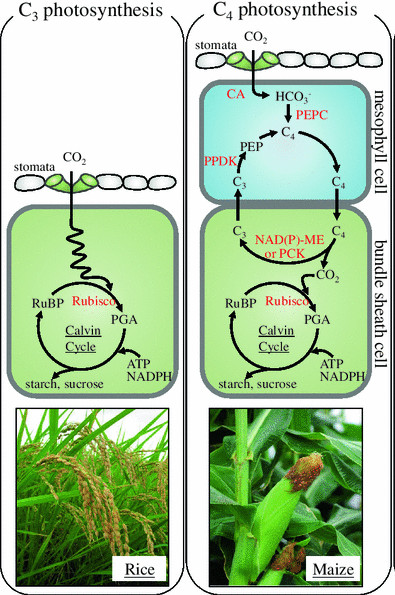
\includegraphics[width=0.9\textwidth]{Figures/c34}
  \end{column}

\end{columns}


\end{frame}
%%%%%%%%%%%


\begin{frame}{Example 1: Does dark respiration differ between C3 and C4 plants?}

    \begin{block}{Can calculate}
 \begin{itemize}
  \item Observed overall mean
  \item Observed mean C3 plants
  \item Observed mean C4 plants
  \item Variation around each mean
 \end{itemize}
\end{block}

\textbf{Statistical model}\\
 DATA = {\color{blue}{Mean for C3}} + {\color{red}{Difference C4-C3}} + {\color{orange}{Noise}}\\
 \pause

 $DATA = {\color{blue}{A}} + {\color{red}{D}} + {\color{orange}{\epsilon}}$
 
 ${\color{blue}{A}} $ and ${\color{red}{D}}$ are the model PARAMETERS. \\
 We want to infer whether ${\color{red}{D}}$ is different from 0

\end{frame}
%%%%%%%%%%%

\begin{frame}{Example 1: Does dark respiration differ between C3 and C4 plants?}
 $DATA = {\color{blue}{A}} + {\color{red}{D}} + {\color{orange}{\epsilon}}$\\

  Can we separate the signal ${\color{red}{D}}$ from the noise ${\color{orange}{\epsilon}}$ ?

 \pause
 
 \begin{block}{T-test}
  \begin{itemize}
   \item Outcome is a continuous variable
   \item Experimental factor is one factor with 2 conditions
   \item No blocking factor / corrections
  \end{itemize}
 \end{block}
 
 \pause
 
 $ t = \frac{\color{red}{D}}{\text{\color{orange}{Variation of }}\color{orange}{\epsilon}} \times \frac{\text{Sample Size}}{\sqrt{2}}$

\end{frame}
%%%%%%%%%%%%

\begin{frame}{When can we know whether $D \neq 0$ ?}

 \begin{columns}
 \begin{column}{0.5\textwidth}
 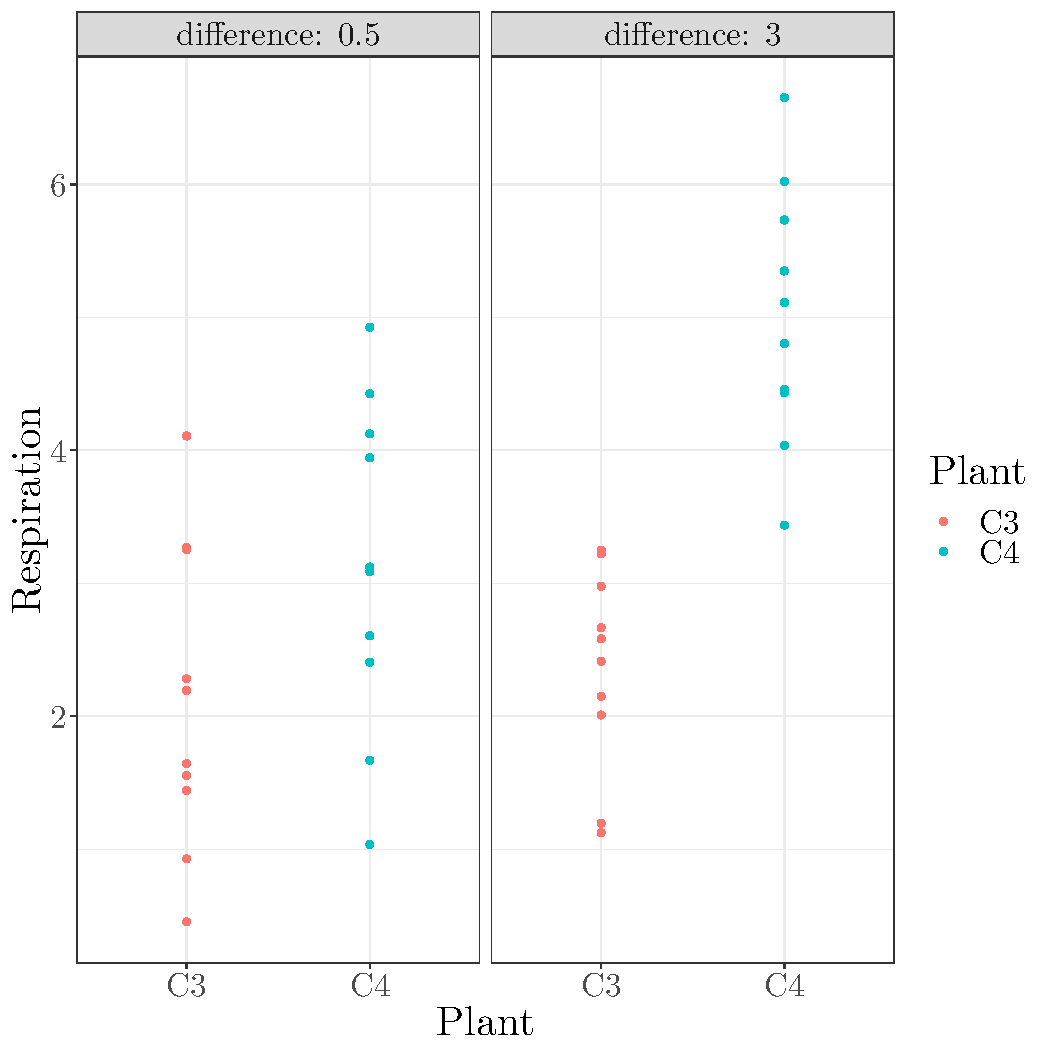
\includegraphics[width=\textwidth]{Figures/figure/ttestdiff-1}
 \end{column}
 \begin{column}{0.5\textwidth}
  $ t = \frac{\color{red}{D}}{\text{\color{orange}{Variation of }}\color{orange}{\epsilon}} \times \frac{\text{Sample Size}}{\sqrt{2}}$

  \vspace{1cm}
  Is it easier when the true difference is 0.5 or when it is 3 ?
 \end{column}
 \end{columns}
 
 \pause
 \begin{alertblock}{}
  \begin{enumerate}
   \item Large true difference between the means
  \end{enumerate}
 \end{alertblock}

\end{frame}
%%%%%%%%%%%

\begin{frame}{When can we know whether $D \neq 0$ ?}

 \begin{columns}
 \begin{column}{0.5\textwidth}
 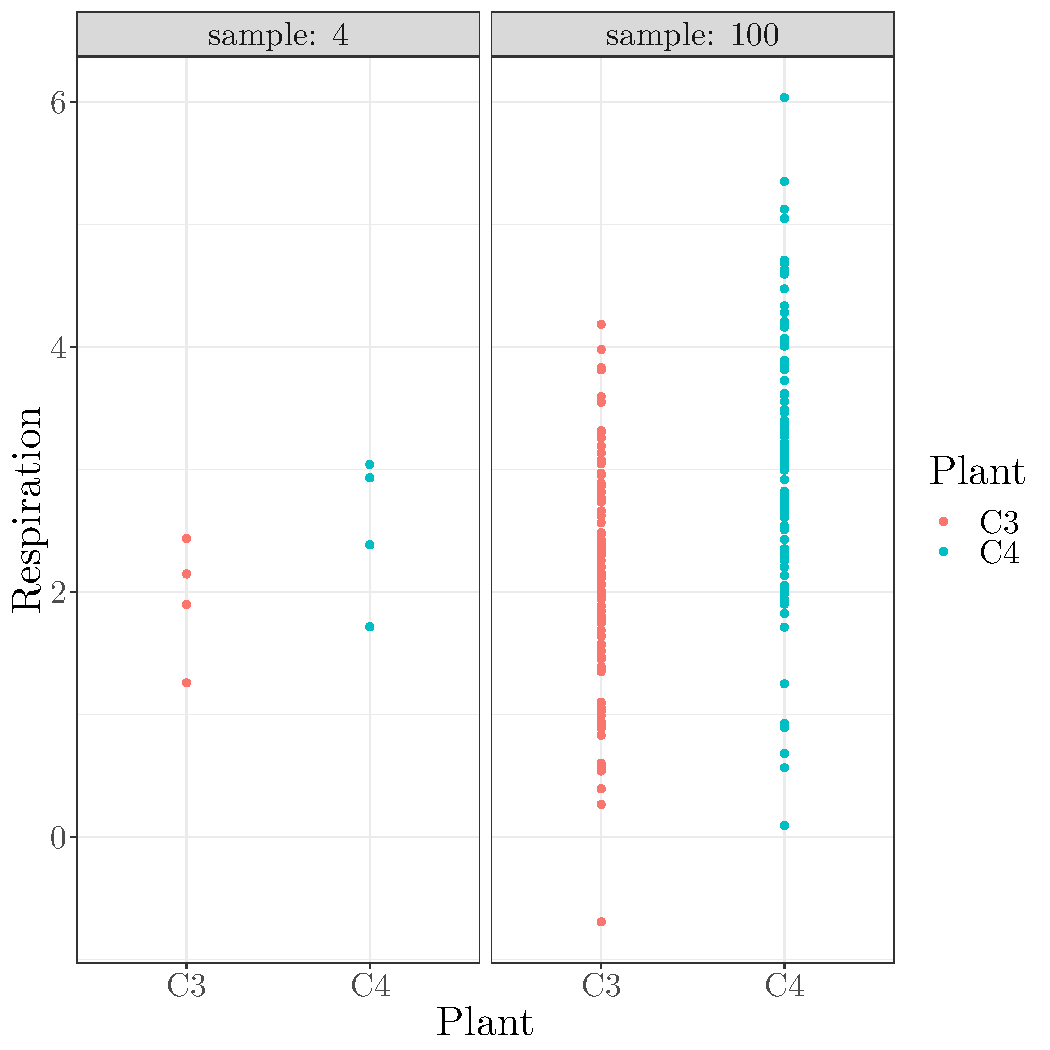
\includegraphics[width=\textwidth]{Figures/figure/ttestsample-1}
 \end{column}
 \begin{column}{0.5\textwidth}
  $ t = \frac{\color{red}{D}}{\text{\color{orange}{Variation of }}\color{orange}{\epsilon}} \times \frac{\text{Sample Size}}{\sqrt{2}}$

  \vspace{1cm}
  Is it easier when sample size is 4 or when it is 100?
 \end{column}
 \end{columns}
 
 \pause
 \begin{alertblock}{}
  \begin{enumerate}
   \item Large true difference between the means
   \item Large sample size
  \end{enumerate}
 \end{alertblock}

\end{frame}
%%%%%%%%%%%


\begin{frame}{When can we know whether $D \neq 0$ ?}

 \begin{columns}
 \begin{column}{0.5\textwidth}
 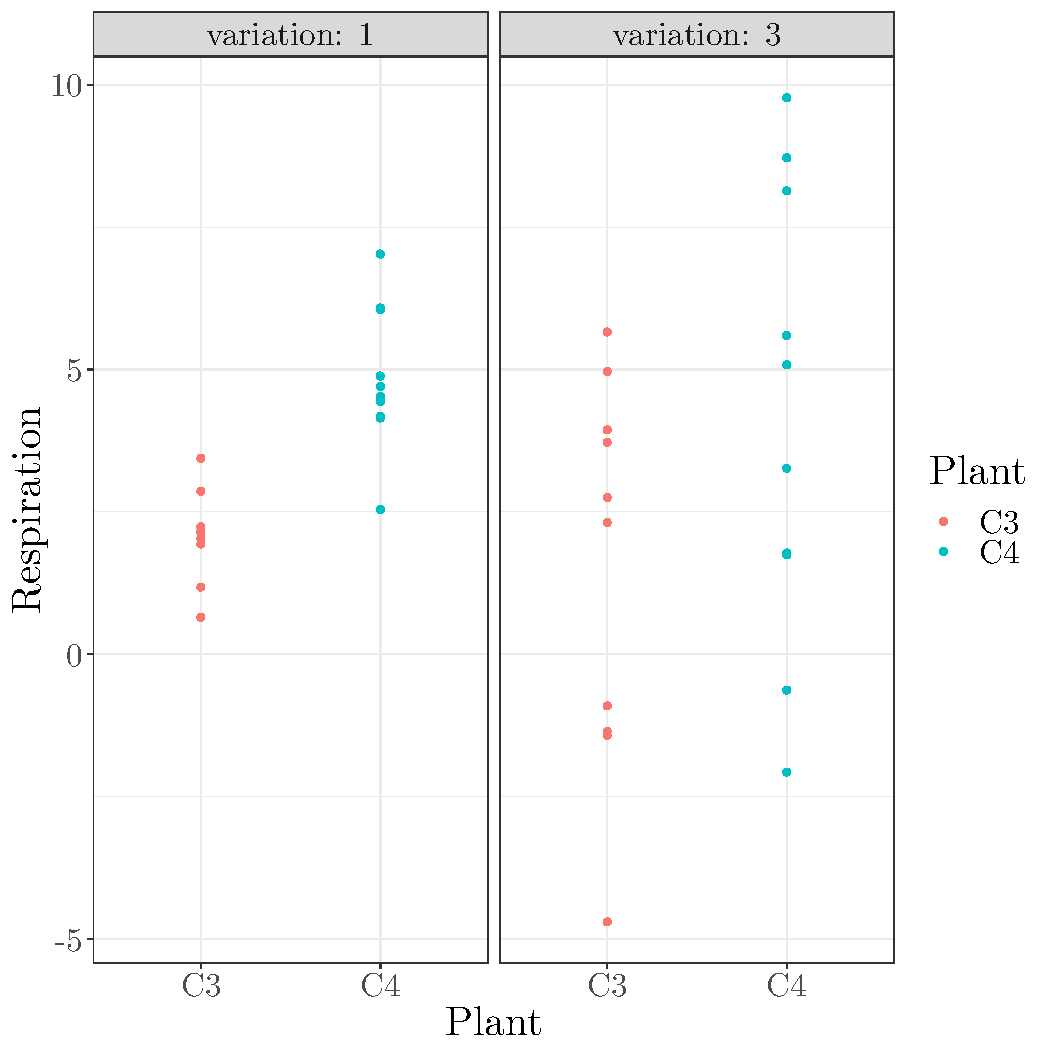
\includegraphics[width=0.9\textwidth]{Figures/figure/ttestvar-1}
 \end{column}
 \begin{column}{0.5\textwidth}
  $ t = \frac{\color{red}{D}}{\text{\color{orange}{Variation of }}\color{orange}{\epsilon}} \times \frac{\text{Sample Size}}{\sqrt{2}}$

  \vspace{1cm}
  Is it easier when unexplained variation is 1 or when it is 3?
 \end{column}
 \end{columns}
 
 \pause
 \begin{alertblock}{What makes $t$ large:}
  \begin{enumerate}
   \item Large true difference between the means
   \item Large sample size
   \item Small unexplained variation
  \end{enumerate}
 \end{alertblock}

\end{frame}
%%%%%%%%%%%



\begin{frame}{When can we know whether $D \neq 0$ ?}
  \centering 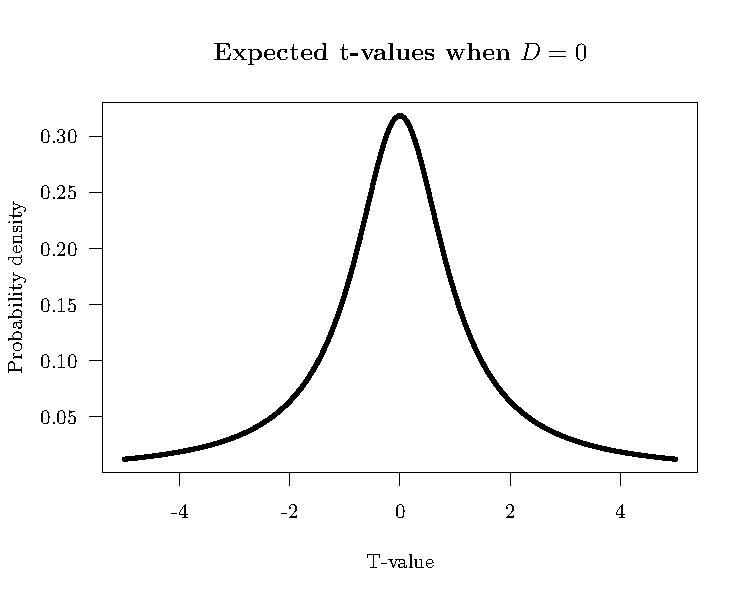
\includegraphics[width=0.7\textwidth]{Figures/figure/tvalue-1}
\end{frame}
%%%%%%%%%%%%


\begin{frame}{When can we know whether $D \neq 0$ ?}
\textbf{p-value}: probability (area under curve) of getting a value as extreme as what you observed, when D=0
\centering  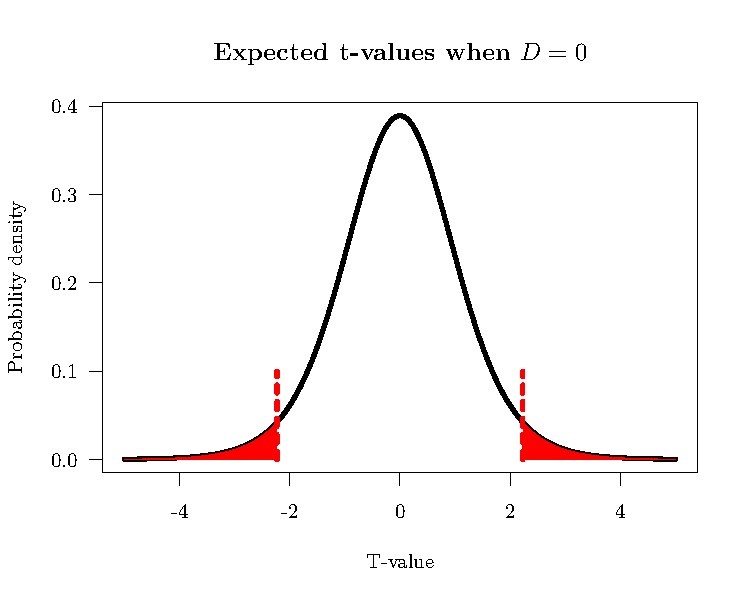
\includegraphics[width=0.7\textwidth]{Figures/figure/tvalueth-1}
\end{frame}
%%%%%%%%%%%%


\begin{frame}{But really, what is a p-value?}
 \begin{block}{Candy practical}
 
 You got 5 Halloween candies out of the bag. Does the bag contain more Halloween than normal candies?
 
 %collect null-distribution data
 %plot in R
 %create null distribution in R
 \end{block}
 
\end{frame}
%%%%%%%%%%%%


\begin{frame}[fragile]{Back to C3/C4 plants. Analyse real data in R}

1. Set working directory (\texttt{setwd(`` / '')}) or create a R-project\\

2. Load and check data
\begin{knitrout}
\definecolor{shadecolor}{rgb}{0.969, 0.969, 0.969}\color{fgcolor}\begin{kframe}
\begin{verbatim}
resp <- read.csv("d_respiration.csv”)
str(resp)
View(resp)
\end{verbatim}
\end{kframe}
\end{knitrout}

3. Visualize data
\begin{knitrout}
\definecolor{shadecolor}{rgb}{0.969, 0.969, 0.969}\color{fgcolor}\begin{kframe}
\begin{verbatim}
library(ggplot2)
ggplot(resp,aes(Plant_type,rrarea,colour=Plant_type))+
    geom_point()+facet_wrap(~Variation)
\end{verbatim}
\end{kframe}
\end{knitrout}

\end{frame}
%%%%%%%%%%%%


\begin{frame}[fragile]{Fit a t-test in R: \texttt{t.test()}}

\textbf{Subset data by Variation (High and Low)}

\begin{knitrout}
\definecolor{shadecolor}{rgb}{0.969, 0.969, 0.969}\color{fgcolor}\begin{kframe}
\begin{verbatim}
resp_H <- subset(resp,Variation == "High")
resp_L <- subset(resp,Variation == "Low")
\end{verbatim}
\end{kframe}
\end{knitrout}

\pause

\textbf{Compare C3 and C4 plants in “High Variation” subset}
\begin{knitrout}
\definecolor{shadecolor}{rgb}{0.969, 0.969, 0.969}\color{fgcolor}\begin{kframe}
\begin{verbatim}
t.test(rrarea~Plant_type, data=resp_H, var.equal=TRUE)
\end{verbatim}
\end{kframe}
\end{knitrout}

\pause
\begin{knitrout}
\definecolor{shadecolor}{rgb}{0.9, 0.9, 0.969}\color{fgcolor}\begin{kframe}
\small
\begin{verbatim}
	Two Sample t-test
data:  rrarea by Plant_type
t = -0.93776, df = 10, p-value = 0.3705
alternative hypothesis: true difference in means is not equal to 0
95 percent confidence interval:
 -1.7619349  0.7181446
sample estimates:
mean in group C3 mean in group C4 
        2.720021         3.241916 
\end{verbatim}
\end{kframe}
\end{knitrout}

\pause $DATA = {\color{blue}{A}} + {\color{red}{D}} + {\color{orange}{\epsilon}}$

\end{frame}
%%%%%%%%%%%

\begin{frame}[fragile]{Fit a t-test in R: \texttt{t.test()}}

\textbf{Compare C3 and C4 plants in “Low Variation” subset}
\begin{knitrout}
\definecolor{shadecolor}{rgb}{0.969, 0.969, 0.969}\color{fgcolor}\begin{kframe}
\begin{verbatim}
t.test(rrarea~Plant_type, data=resp_L, var.equal=TRUE)
\end{verbatim}
\end{kframe}
\end{knitrout}

\end{frame}
%%%%%%%%%%%

\begin{frame}[fragile]{Fit an anova in R: \texttt{aov()}}

\begin{knitrout}
\definecolor{shadecolor}{rgb}{0.969, 0.969, 0.969}\color{fgcolor}\begin{kframe}
\begin{verbatim}
aov1 <- aov(rrarea~Plant_type, data=resp_H)
summary(aov1)
\end{verbatim}
\end{kframe}
\end{knitrout}

\vspace{-0.15cm}
\pause
\begin{knitrout}
\definecolor{shadecolor}{rgb}{0.9, 0.9, 0.969}\color{fgcolor}\begin{kframe}
\footnotesize
\begin{verbatim}
            Df Sum Sq Mean Sq F value Pr(>F)
Plant_type   1  0.817  0.8171   0.879   0.37
Residuals   10  9.292  0.9292  
\end{verbatim}
\end{kframe}
\end{knitrout}

\pause $DATA = {\color{blue}{A}} + {\color{red}{D}} + {\color{orange}{\epsilon}}$

\end{frame}
%%%%%%%%%%%

\begin{frame}[fragile]{Fit a linear model in R: \texttt{lm()}}

\begin{knitrout}
\definecolor{shadecolor}{rgb}{0.969, 0.969, 0.969}\color{fgcolor}\begin{kframe}
\begin{verbatim}
lm1<-lm(rrarea ~ Plant_type, data = resp_L)
summary(lm1)
\end{verbatim}
\end{kframe}
\end{knitrout}

\vspace{-0.15cm}
\pause
\begin{knitrout}
\definecolor{shadecolor}{rgb}{0.9, 0.9, 0.969}\color{fgcolor}\begin{kframe}
\footnotesize
\begin{verbatim}
lm(formula = rrarea ~ Plant_type, data = resp_H)

Residuals:
    Min      1Q  Median      3Q     Max 
-1.7380 -0.4201 -0.1437  0.6706  1.6754 

Coefficients:
             Estimate Std. Error t value Pr(>|t|)    
(Intercept)    2.7200     0.3935   6.912 4.13e-05 ***
Plant_typeC4   0.5219     0.5565   0.938     0.37    
---
Signif. codes:  0 ‘***’ 0.001 ‘**’ 0.01 ‘*’ 0.05 ‘.’ 0.1 ‘ ’ 1

Residual standard error: 0.9639 on 10 degrees of freedom
Multiple R-squared:  0.08083,	Adjusted R-squared:  -0.01109 
F-statistic: 0.8794 on 1 and 10 DF,  p-value: 0.3705
\end{verbatim}
\end{kframe}
\end{knitrout}

\pause $DATA = {\color{blue}{A}} + {\color{red}{D}} + {\color{orange}{\epsilon}}$

\end{frame}
%%%%%%%%%%%

\begin{frame}[fragile]{Fit a linear model in R: \texttt{lm()}}

\begin{knitrout}
\definecolor{shadecolor}{rgb}{0.969, 0.969, 0.969}\color{fgcolor}\begin{kframe}
\begin{verbatim}
library(emmeans)
emmeans(lm1, ~Plant_type)
\end{verbatim}
\end{kframe}
\end{knitrout}


\begin{knitrout}
\definecolor{shadecolor}{rgb}{0.9, 0.9, 0.969}\color{fgcolor}\begin{kframe}
\footnotesize
\begin{verbatim}
 Plant_type   emmean        SE df lower.CL upper.CL
 C3         2.720021 0.3935305 10 1.843180 3.596861
 C4         3.241916 0.3935305 10 2.365076 4.118757

Confidence level used: 0.95 
\end{verbatim}
\end{kframe}
\end{knitrout}

\pause $DATA = {\color{blue}{A}} + {\color{red}{D}} + {\color{orange}{\epsilon}}$

\end{frame}
%%%%%%%%%%%

\begin{frame}{Compare the output from t.test, aov and lm}
 
\end{frame}
%%%%%%%%%%%%


\begin{frame}{}
 
\end{frame}
%%%%%%%%%%%%


\begin{frame}{All is one\dots}
\pause
  \begin{block}{\dots but \texttt{lm()} rules!}
    \begin{itemize}
      \item t-test, ANOVA, regression and others can be mathematically equivalent
      \item In R, \texttt{lm()} and related functions can do them all\dots
      \item \dots and much more!
    \end{itemize}
  \end{block}
\end{frame}
%%%%%%%%%%%


% more on LM, general steps, and another example

\end{document}
